%%%%%%%%%%%%%%%%%%%%%%%%%%%%%%%%%%%%%%%%%%%%%%%%%%%%%%%%%%%%%%%%%%%%%%%%%%%%%%%%
%%                           ONDER DE LOEP ARTIKEL                            %%
%%%%%%%%%%%%%%%%%%%%%%%%%%%%%%%%%%%%%%%%%%%%%%%%%%%%%%%%%%%%%%%%%%%%%%%%%%%%%%%%
\artikel{Spreidingsdiagrammen en trendlijnen}{Statistiek in de 2$^\text{e}$ graad}{Johan Deprez\\Filip Moons}

\startcontents[inhoudloep]	% om inhoud voor het loep artikel te beginnen

\begin{multicols}{2}
	
	\inhoudstafelloep			% om inhoudstafel voor het loep artikel te tonen
	\vspace{-5mm}
	%% Gebruik \section{titel} en \subsection{titel} om genummerde tussentitels te maken
	\section{Inleiding}
Wie aan eerstegraadsfuncties denkt, denkt meteen aan oefeningetjes zoals: 	
\begin{citaat}
     Richard \& Els geven een trouwfeest. Voor het avondfeest vraagt de trouwlocatie 1950 EUR voor het gebruik van de zaal en 89 EUR per aanwezige. Bepaal de vergelijking van de rechte die de totale prijs $y$ uitzet tegenover het aantal aanwezigen $x$.
         \end{citaat}	

Maar wat als de vraag als volgt luidt:

\begin{citaat}
     Een klas van 18 leerlingen legde twee wiskundetoetsen op 10 punten af: één in september en één in december. De punten werden uitgezet op onderstaande grafiek. Op de $x$-as staan de scores van september, op de $y$-as de scores van december. Bepaal de vergelijking van een rechte die de trend in de puntenwolk beschrijft.
    \end{citaat}
\afbeelding[0.8\textwidth]{img/Lregressie_wiskundetoets.png}{Spreidingsdiagram}{spreid}
Twee keer dezelfde vraag (`Bepaal de vergelijking van een rechte'), maar toch twee keer een totaal verschillend antwoord. In het voorbeeld van het trouwfeest valt de vergelijking rechtstreeks te bepalen: de opstartkost van 1950 EUR  komt overeen met het intercept (snijpunt $y$-as), de prijsstijging per extra aanwezige is de richtingscoëfficiënt. We bekomen dus $y = 1950 + 89x$. Elk mogelijk puntenkoppel van aantal aanwezigen en totaalprijs, bv. $(100,10850)$ zal ook op de rechte liggen. We spreken van een \textit{functionele relatie} tussen de variabelen `aantal aanwezigen' en `totaalprijs.' 

In het voorbeeld van de wiskundetoetsen is het functievoorschrift van de trendlijn niet exact te bepalen. De puntenwolk suggereert wel een trend: wie hoog scoorde op de wiskundetoets in september, scoorde doorgaans ook hoog op de wiskundetoets in december. Toch geldt dat niet voor alle leerlingen: zo is er een leerling die van een 8/10 in september, naar een magere 4/10 duikelt in december. De punten zullen dus verspreid rond de trendlijn liggen. Vandaar dat we grafieken zoals in \autoref{spreid2} \textit{spreidingsdiagrammen} noemen. 

De spreiding van die punten wijst erop dat er variatie bestaat in de scores op de decembertoets die niet kan geassocieerd worden met de scores op de septembertoets. Vermits de score op de wiskundetoets in december niet exact te bepalen valt op basis van de score op de wiskundetoets in september, spreken we van een \textit{statistische relatie} tussen de variabelen `score september' en `score december'. Excel levert als vergelijking van de trendlijn $y = 0,69x + 1,60$. Wie een 5 haalde op de wiskundetoets in september, kan volgens dit model een $0,69\cdot5+1,60 = 5,05$ verwachten in december.
\afbeelding[0.8\textwidth]{img/Lregressie_wiskundetoets2.png}{Spreidingsdiagram met trendlijn}{spreid2}
Spreidingsdiagrammen en trendlijnen zijn een stukje bivariate statistiek: je legt het verband tussen twee variabelen, zoals bv. de wiskundescores in september en december. Dit is nieuw in de eindtermen van de tweede graad doorstroomfinaliteit. Univariate beschrijvende statistiek, waarbij je frequentietabellen, histogrammen en boxplots opstelt en gemiddeldes/standaardafwijkingen berekent van één variabele (bv. de schoenmaten in de klas), waren al langer vaste prik in de tweede graad.

Het onderwerp zit op de grens tussen statistiek en functieleer en het vormt een uitstekende gelegenheid om in te gaan op het gebruik van functies als wiskundig model voor fenomenen uit de realiteit. Hierdoor sluit het mooi aan bij de eerstegraadsfuncties in de tweede graad en bij de wetenschapsvakken. Vermits leerlingen al een inleiding op univariate beschrijvende statistiek achter de kiezen hebben in de hervormde eerste graad en het stuk steekproef versus populatie naar de derde graad is verschoven, was er ook ruimte voor. De eindterm rond spreidingsdiagrammen en trendlijnen legt daarnaast de link met de veelvoorkomende misvatting dat een correlatie een causaal verband impliceert. Door een uitstapje naar niet-lineaire trendlijnen aan te bieden, wil de eindterm ook vermijden dat leerlingen opgezadeld zitten met het misconcept dat alle statistische verbanden tussen twee variabelen lineair zijn. Al deze thema's komen aan bod in deze loep.

Belangrijk om in het achterhoofd te houden, is dat alle statistiek tot en met de tweede graad uitsluitend beschrijvend van aard is. Dat is ook de reden waarom het stukje `steekproef versus populatie' bewust naar de derde graad is verschoven: het is de noodzakelijke inleiding op `inferentiële statistiek', waarbij je op basis van data van een steekproef, uitspraken wil doen voor de volledige populatie en dit hoort dus helemaal niet bij beschrijvende statistiek. In wetenschappelijk onderzoek zijn de puntenwolken waarbij je een trendlijn bepaalt, bijna altijd data uit een steekproef. De trendlijn die je bekomt, moet representatief zijn voor de populatie. De waarden van het intercept en de richtingscoëfficiënt zijn schattingen van de populatiewaarden op basis van die steekproefdata. Door die onzekerheid worden ze vaak samen met hun betrouwbaarheidsintervallen gerapporteerd. Daarnaast bestaan er significantietoetsen om na te gaan of de richtingscoëfficiënt significant verschilt van nul of niet (m.a.w.: blijkt uit de data een significante trend of niet?). Dit valt echter ver buiten het bestek van de tweede graad. Zelfs in de derde graad zou dit uitbreidingsleerstof zijn: betrouwbaarheidsintervallen en hypothesetoetsen zijn verplicht voor sommige richtingen, maar niet in de context van lineaire regressie. Dit duidt wel mooi hoe de leerlijn statistiek is opgevat in de volledige doorstroomfinaliteit.
	\section{Spreidingsdiagrammen}
Een spreidingsdiagram is een grafiek die in de vorm van een puntenwolk de samenhang tussen twee variabelen $x$ en $y$ weergeeft. Elk koppel uit een verzameling van waarnemingswaarden $(x_1,y_1 ),(x_2,y_2 ),\ldots,(x_n,y_n)$ wordt gepresenteerd door een punt in een assenstelsel en de dataset geeft zo een puntenwolk die bestaat uit $n$ observaties. De verspreiding of samenklontering van de punten geeft weer of en hoe de variabelen $x$ en $y$ samenhangen. Door deze puntenwolk te bestuderen, kun je vaststellen of er een verband bestaat tussen deze twee variabelen, en als er een verband is, kun je ook de aard ervan bepalen (recht evenredig, omgekeerd evenredig, lineair, kwadratisch$\ldots$). 
\end{multicols}

 \afbeelding{img/LRegressie_economist.png}{Spreidingsdiagram uitgaven aan kerstcadeaus}{fig:economist}
\begin{multicols}{2}
Een voorbeeld van zo’n spreidingsdiagram vinden we in  \autoref{fig:economist}, afkomstig uit The Economist (12 December, 2011) over de uitgaven aan kerstcadeaus in verschillende landen. Op de $x$-as vinden we de verwachte uitgave aan kerstcadeaus terug in dollar, op de $y$-as het BBP (Bruto Binnenlands Product) per persoon. Het BBP per persoon geeft aan hoe rijk een land is. Elk punt in de puntenwolk stelt een land voor. Naarmate een land hoger ligt, is het rijker. Naarmate een land meer naar rechts ligt, geven mensen gemiddeld meer uit aan kerstcadeaus. 

We merken op dat inwoners van rijkere landen (VS, Ierland, Zwitserland,$\ldots$) doorgaans meer uitgeven aan kerstcadeaus dan inwoners in armere landen (Oekraïne, Zuid-Afrika, Polen \dots). Er lijkt globaal genomen sprake van een recht evenredig verband. 

Daarnaast vallen twee punten op die afwijken van het patroon: Nederland en Luxemburg. Zij gedragen zich anders dan de andere landen en volgen niet dezelfde trend. Nederlanders lijken minder uit te geven aan kerstcadeaus dan ze volgens hun rijkdom gemiddeld zouden kunnen. Luxemburgers geven het meest uit aan kerstcadeaus, maar het punt volgt niet dezelfde trend dan de andere punten: in vergelijking met hun rijkdom geven Luxemburgers weinig uit aan kerstcadeaus. Deze punten roepen vragen op: wat is er met deze landen aan de hand? Klopt het cliché dat Nederlanders gieriger zijn? Is er bij Luxemburgers ergens een `psychologische' uitgavelimiet die men niet wil overschrijden ondanks dat de gemiddelde Luxemburger zich best wel duurdere kerstcadeaus kan permitteren?
\begin{figure*}
 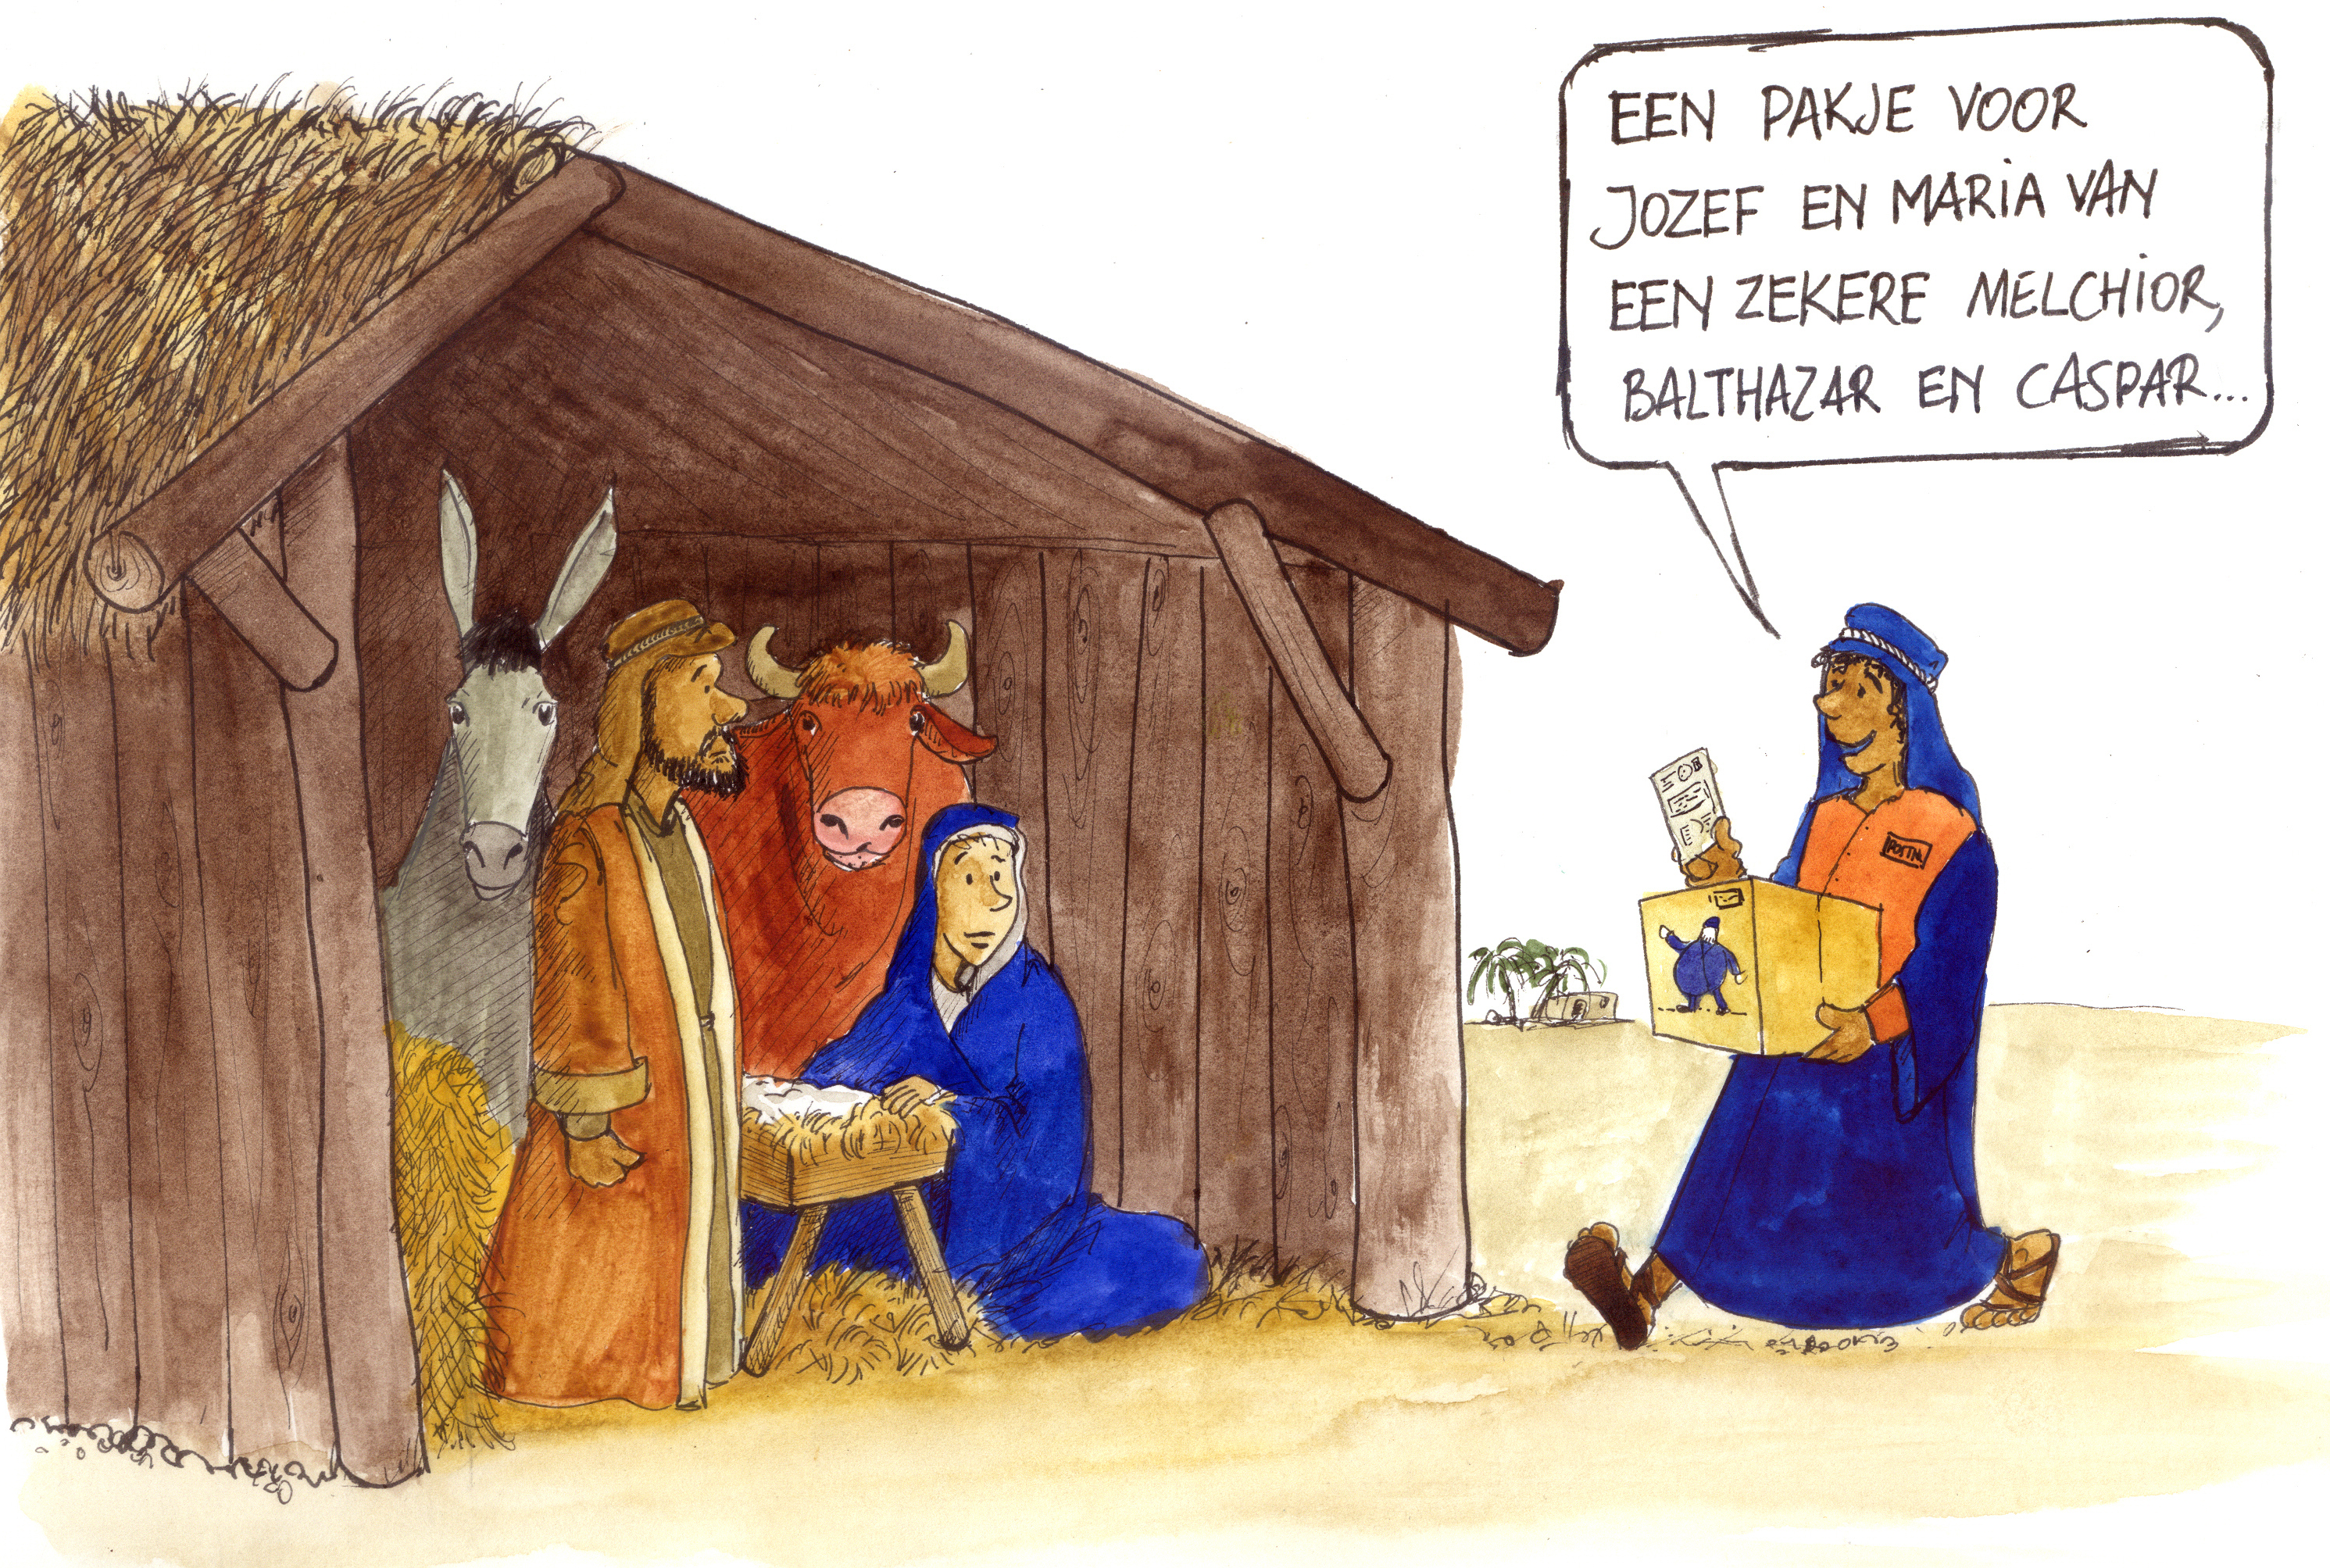
\includegraphics[width=1\textwidth]{tekeningenKurt/uw stal.jpg}
\end{figure*}
Uit voorgaand voorbeeld blijkt meteen het nut van een spreidingsdiagram: het is meestal de eerste stap om samenhang tussen twee variabelen te bestuderen waarbij een mogelijke samenhang, de aard van het verband en punten die het patroon niet volgen meteen allerlei vragen oproepen. Het spreidingsdiagram geeft alleen een eerste, beschrijvend idee en geen verklaringen: de grafiek roept op tot nader onderzoek.

In het begin van de lessenreeks moet de focus vooral op het correct interpreteren van spreidingsdiagramman liggen. We geven een aantal maatschappelijk relevante voorbeelden via een lesactiviteit.

\end{multicols}
\begin{lesactiviteit}{Interpreteren van spreidingsdiagrammen}

\textbf{Rijkdom versus jongeren die niets doen}

Eurostat, het bureau voor de statistiek van de Europese Unie heeft met `Regions and Cities Illustrated' (RCI) een online tool beschikbaar via https://ec.europa.eu/eurostat/cache/RCI/. Hiermee kun je tal van variabelen tegenover elkaar uitzetten in een spreidingsdiagram. 

Bekijk de grafiek in  onderstaande figuur. Deze bevat iets meer informatie dan een traditioneel spreidingsdiagram: de kleuren onderlijnen de $x$-waarde (die dan uitgezet worden op de kaart van Europa), de grootte van de bollen geeft de populatiegrootte. Zoek eventueel extra informatie via internet en beantwoord volgende vragen:

\begin{vraagenantwoord} 
\vraag{Wat stelt een punt voor in deze puntenwolk?} 
\antwoord{Elk punt stelt een Europese regio voor.}
\vraag{Tussen welke statistische variabelen wordt gezocht naar samenhang? Zoek op internet eventueel naar extra informatie.} 
\antwoord{De samenhang tussen het BBP (Bruto Binnenlands Product) per persoon enerzijds en het aandeel jongeren (tussen 15-24 jaar) dat noch werkt, noch enige vorm van onderwijs geniet. Het BBP/persoon is een maat voor de rijkdom van een land.} 
\vraag{Welke variabelen staan op welke assen en hoe zijn ze uitgedrukt?}
\antwoord{$x$-as: percentage 15 tot 24-jarigen dat noch werkt, noch enige vorm van opleiding geniet\\$y$-as: BBP per persoon in euro.}
\vraag{Welk patroon merk je op voor de meeste punten?}
\antwoord{Hoe lager het aandeel jongeren (tussen 15-24 jaar) dat noch werkt, noch enige vorm van onderwijs geniet, hoe rijker de regio. Er is sprake van een \aanh{hoe hoger $\ldots$ hoe lager $\ldots$}-verband of een negatief lineair verband.}
\vraag{Zijn er punten die de algemene trend niet lijken te volgen? Kun je hiervoor een mogelijke verklaring bedenken?}
\antwoord{Ja, Brussel heeft voor zijn hoge aandeel `nietsdoende' jongeren (13$\%$) een hoog BBP/persoon. Andere regio's met een gelijkaardig aandeel `nietsdoende' jongeren zijn doorgaans veel armer.  Luxemburg heeft een vrij laag aandeel `nietsdoende' jongeren maar is gemiddeld genomen rijker dan regio's met een gelijkaardig aandeel. Eenzelfde fenomeen treedt op voor Zuid-Ierland: de regio is rijker dan men zou verwachten op basis van het aandeel `nietsdoende' jongeren. In Luxemburg zorgt de aanwezigheid van financiële instellingen allicht voor de hogere rijkdom, in Brussel zou het kunnen liggen aan de aanwezigheid van internationale instellingen en Zuid-Ierland is mogelijk rijker door toerisme.}
\end{vraagenantwoord}
\begin{center}
  \includegraphics[width=0.99\linewidth]{img/LRegressie_eurostat.png} 
\end{center}
 
\end{lesactiviteit}


\begin{multicols}{2}
\subsection{Keuze en schaling van de assen}
Om te bepalen welke variabele op de $x$-as hoort en welke op de $y$-as bij een spreidingsdiagram, is het doorgaans gebruikelijk om de `verklarende variabele' (= onafhankelijke variabele) op de $x$-as te plaatsen en de `responsvariabele' (=afhankelijke variabele) op de $y$-as. Bij het voorbeeld met de wiskundetoetsen in \autoref{spreid2} willen we de score in december (responsvariabele, $y$-as) bepalen aan de hand van de score in september (verklarende variabele, $x$-as). \afbeelding[1\textwidth]{img/Lregressie_econ2.jpg}{Voorbeeld uit The Economist met verwisselde assen}{econ2}
Merk op dat het voorbeeld over de uitgaven aan kerstcadeaus in \autoref{fig:economist} deze conventie niet volgt: de meeste mensen gaan immers de uitgaven aan kerstcadeaus willen verklaren aan de hand van het BBP/persoon, waardoor het logischer zou zijn om de uitgave aan kerstcadeaus als responsvariabele op de $y$-as te plaatsen en het BBP als verklarende variabele op de $x$-as. Dit levert een spreidingsdiagram op zoals in \autoref{econ2} waarbij de punten gespiegeld zijn tegenover de eerste bissectrice (let op: de $x$- en $y$-as zijn niet gelijk geschaald). Deze figuur maakt duidelijk dat de redactie van The Economist allicht bewust de conventie niet volgde omdat de lay-out zo mooier uitviel. Hoewel het voor een spreidingsdiagram bij een lineaire trend louter een conventie betreft wat op de $x$-as en wat op de $y$-as komt, is het wel een belangrijke keuze om de trendlijn te bepalen.

De schaling van de assen op een spreidingsdiagram zijn doorgaans verschillend. Meestal neemt men als schaling het waardenbereik van de gegevens (met een klein beetje extra ruimte aan de uiteinden, zodanig dat er geen punten tegen de randen plakken).  Als een variabele een natuurlijk nulpunt heeft, dan hoort de as te beginnen bij dat nulpunt. Beginnen bij een waarde groter dan 0 kan een vertekend beeld opleveren, al is het soms wel nodig om een trend te kunnen zien. Een valide, niet-misleidende schaling hangt altijd af van de context van het probleem.  Wie grafieken plot met een spreadsheetprogramma, krijgt standaard meestal meteen een goede schaling van de assen voorgesteld. 


\subsection{Naamgeving}
De naam \aanh{spreidingsdiagram} is in het Nederlands een beetje ongelukkig gekozen. De spreiding duidt immers op de \textit{verspreiding} van de punten op de grafiek en rond de trendlijn (indien die getekend is). Die verspreiding heeft niets te maken met de spreidingsmaten (standaardafwijking, variatiebreedte, interkwartielafstand $\ldots$) die leerlingen bij één veranderlijke bestudeerden in de tweede graad. In het Engels heeft men twee verschillende woorden voor dat betekenisverschil en spreekt men dan ook van een \textit{scatter plot} en niet van een \textit{spread plot}. Ook het Nederlands heeft een aantal minder verwarrende synoniemen: zo wordt een spreidingsdiagram ook wel een strooiingsdiagram, een puntenwolk, een puntdiagram of correlatiediagram genoemd. 
Sommigen noemen een histogram/staafdiagram onterecht een spreidingsdiagram in de zin van een ‘diagram dat toont hoe de gegevens gespreid zijn.' Dat klopt niet: histogrammen en staafdiagrammen beschrijven de verdeling van gegevens van één veranderlijke (= univariaat) en heeft dus niets te maken met een spreidingsdiagram (= bivariaat).


	\section{Rechte als trendlijn}

Nu we spreidingsdiagrammen geïntroduceerd hebben, is het tijd om over te stappen naar trendlijnen. We starten met lineaire trendlijnen. We hebben over dit onderwerp in het verleden al een aantal keer geschreven in Uitwiskeling (Deprez, Op de Beeck, Van den Broeck, 2011; Deprez, Roels, Tytgat, 2005; Deprez, Vanlommel, 2020). In deze paragraaf vind je nieuw materiaal, maar soms nemen we ook onderdelen uit dat oudere materiaal over en passen we het in een opgefriste vorm in deze nieuwe loep in. In de eerdere teksten vind je dan vaak nog bijkomende uitgewerkte voorbeelden. We plaatsen deze oudere teksten ook integraal op onze website, niet alleen in het nummer in kwestie, maar ook als bijlage als je deze loep online consulteert.

   \subsection{Eerstegraadsfuncties met context} \label{section:eerstegraadsfuncties met context}
   
In het derde jaar worden eerstegraadsfuncties bestudeerd. Dat gebeurt deels contextloos, maar eerstegraadsfuncties duiken ook op in allerlei toepassingen. Zo beschrijft de eerstegraadsfunctie $T_F=32+1,8 \cdot T_C$ bijvoorbeeld het verband tussen de temperatuur van een voorwerp in graden Fahrenheit ($T_F$) en in graden Celsius ($T_C$) (zie ook Deprez en Vanlommel, 2020).

De vergelijking uit de vorige alinea kan het startpunt zijn van een oefening of een voorbeeld, maar je kunt leerlingen ook vragen om de vergelijking zelf op te stellen. Als vertrekpunt moet je dan bijvoorbeeld weten dat het verband tussen $T_F$ en $T_C$ van de eerste graad is en dat water bevriest bij 32 graden Fahrenheit en kookt bij 212 graden Fahrenheit. Immers, een eerstegraadsfunctie ligt volledig vast als je twee van zijn koppels kent. Of, in meetkundige termen: een rechte wordt volledig bepaald door twee punten.

De vergelijking, of de grafiek, mag in elk geval niet het eindpunt zijn van de oefening of het voorbeeld. Het is bijvoorbeeld goed om even stil te staan bij de betekenis van de twee coëfficiënten in de vergelijking. De constante term of intercept bepaalt het snijpunt met de verticale as. De richtingscoëfficiënt drukt uit dat een stijging van de temperatuur met één graad Celsius overeenkomt met een stijging met $1,8$ graden Fahrenheit. En je kunt in deze context allerlei (zinvolle) vragen bedenken die aanleiding geven tot het oplossen van vergelijkingen.

   \subsection{Van zuivere wiskunde naar rechte als wiskundig model: de eerste stappen}

In het voorbeeld uit de voorgaande paragraaf gebruiken we eerstegraadsfuncties in een toegepaste context, maar blijft de eerstegraadsfunctie een \emph{exacte} beschrijving van het fenomeen uit de realiteit. Dat betekent dat gekende eigenschappen, zoals ‘twee punten bepalen juist één rechte’, hier nog onverkort gebruikt kunnen worden (zoals we dat in het temperatuursvoorbeeld ook gedaan hebben). Het komt echter veel vaker voor dat de realiteit enkel \emph{benaderend}, en niet exact, door een eerstegraadsfunctie beschreven kan worden. De eerstegraadsfunctie wordt dan gebruikt als een wiskundig model dat de realiteit benaderend of geïdealiseerd weergeeft. Dat is een stap die je expliciet met de leerlingen moet maken.

In Deprez e.a. (2011) hebben we een voorbeeld uitgewerkt waarin deze stap gezet wordt in de context van het drukken van een flyer waarbij de prijs afhangt van de bestelde hoeveelheid. Voor een eerste type van folder worden de prijzen gegeven in \autoref{tab:flyer01}.

	\begin{tabel}
		\begin{tabular}{C{3.9cm} C{3.2cm}}
			\hlinethick
			\tableheader{bestelde hoeveelheid (in eenheden van 1000 exemplaren)} & \tableheader{prijs (in EUR)} \\
			\hlinethick
            1 & 125 \\
            2 & 146 \\
            3 & 167 \\
            4 & 188 \\
            5 & 209 \\
			\hlinethick
		\end{tabular}
		\caption{Prijs voor drukwerk voor een eerste type flyer}\label{tab:flyer01}
	\end{tabel}

Het verband tussen de hoeveelheid (in eenheden van 1000 exemplaren, $x$) en de prijs (in EUR, $p$) wordt exact beschreven door de eerstegraadsfunctie met vergelijking $p=104+21x$.

Bij een ander formaat worden de prijzen gegeven in \autoref{tab:flyer02}.

	\begin{tabel}
		\begin{tabular}{C{3.9cm} C{3.2cm}}
			\hlinethick
			\tableheader{bestelde hoeveelheid (in eenheden van 1000 exemplaren)} & \tableheader{prijs (in EUR)} \\
			\hlinethick
            1 & 99 \\
            2 & 120 \\
            3 & 142 \\
            4 & 163 \\
            5 & 183 \\
			\hlinethick
		\end{tabular}
		\caption{Prijs voor drukwerk voor een tweede type flyer}\label{tab:flyer02}
	\end{tabel}

De situatie is nu minder duidelijk. De supplementaire kost voor een bijkomende eenheid is niet altijd dezelfde: achtereenvolgens $21$, $22$, $21$ en $20$ EUR. Daaruit kunnen we afleiden dat de vijf punten niet op één rechte liggen. Er is dus geen eerstegraadsvergelijking die de prijs geeft in termen van het aantal exemplaren. Je zou het daar bij kunnen laten. Als je echter naar \autoref{fig:flyer02A} kijkt, zie je dat de punten \emph{bijna} op één rechte liggen.

	\afbeelding{img/Lregressie_JD_flyer02A.png}{Prijs voor drukwerk voor een tweede type flyer}{fig:flyer02A} 

Hoewel we dus geen eerstegraadsvergelijking meer hebben die de exacte prijzen geeft, kunnen we wel een eerstegraadsvergelijking vinden die de prijzen \emph{bij benadering} beschrijft. Je kunt bijvoorbeeld gebruik maken van het eerste en laatste van de vijf punten. \autoref{fig:flyer02B} toont de rechte door deze twee punten.

	\afbeelding{img/Lregressie_JD_flyer02B.png}{Prijs voor drukwerk voor een tweede type flyer met rechte}{fig:flyer02B} 

Als vergelijking voor de eerstegraadsfunctie vind je dan $p=21x+78$ . Deze formule geeft ons een goed idee van de prijs van het drukwerk: voor een hoeveelheid van $1$, $2$ en $5$ eenheden geeft ze de correcte prijs en voor $3$ en $4$ eenheden zit ze er amper $1$ EUR naast.

De moraal van het verhaal is dat we nog altijd gebruik kunnen maken van een eenvoudige formule om de tabel samen te vatten, tenminste als we ons tevreden kunnen stellen met benaderende waarden voor de prijzen. Deze manier van werken staat haaks op wat we gewoon zijn binnen de \emph{zuivere wiskunde}, maar \emph{in de praktijk} is het heel vaak zo dat we tevreden zijn met een eenvoudige formule die de realiteit benaderend beschrijft. Zo’n eenvoudige formule wordt dan een \emph{wiskundig model} genoemd.

We vinden het belangrijk om deze stap expliciet te benoemen voor leerlingen. Er wordt een ander kader geschapen, waarin andere regels gelden: in het kader van de zuivere wiskunde zou het fout zijn om te zeggen dat het verband tussen prijs en aantal beschreven wordt door een eerstegraadsfunctie, terwijl het in het kader van het wiskundig modelleren juist wel gerechtvaardigd is. Of het juist of fout is, hangt dus van de context af.

De formule hierboven is niet de enige mogelijkheid. Je zou de rechte bijvoorbeeld een halve eenheid naar boven kunnen schuiven en dus gebruik maken van de formule $p=21x+78,5$. Je zit dan drie keer $0,5$ EUR boven en twee keer $0,5$ EUR onder de prijs uit de tabel. Het is de moeite waard om beide formules met elkaar te vergelijken. Een nadeel van de nieuwe formule is dat ze de prijs geen enkele keer helemaal juist weergeeft. De oude formule zat drie keer juist, maar twee keer te laag. Ze zit dus gemiddeld te laag. De tweede formule zit drie keer te hoog en twee keer te laag. Gemiddeld gezien zit ze maar een klein beetje hoger dan de werkelijke kostprijs. Bovendien is het verschil met de waarden in de tabel in absolute waarde nu nooit groter dan $0,5$ EUR.

We stellen dus vast dat er nu niet meer één ‘juiste’ vergelijking is, maar dat er meerdere formules te bedenken zijn en dat er voor elk van die formules wel goede argumenten te geven zijn. Ook dat is anders dan in de zuivere wiskunde, waar er bij één vraag altijd juist één goed antwoord is.

Bemerk dat we de rechte(n) of eerstegraadsfunctie(s) hier `enkel met ons gezond verstand' bepaald hebben. We hebben dat bewust gedaan. We denken dat het goed is om dat in het begin enkele keren zo te doen. Op die manier is er niets geheimzinnigs aan deze rechte, en het helpt ook om in te zien dat we een wiskundig model niet mogen verabsoluteren.

    \subsection{De trendlijn bepalen met ICT}

We blijven natuurlijk niet steken bij het bepalen van de trendlijn `enkel met ons gezond verstand', zoals op het einde van de vorige paragraaf aangegeven: het kost bijvoorbeeld veel tijd om de vergelijking op te stellen en het is vervelend dat we allemaal bij een licht verschillende rechte kunnen uitkomen. In veel ICT-tools is een algoritme ingebouwd waarmee in een oogwenk een eenduidige trendlijn bepaald kan worden.

Met de grafische rekenmachine TI84 maak je gebruik van het commando LinReg(ax+b) of LinReg(a+bx) uit het STAT-CALC-menu (zie \autoref{fig:flyer02C}).

\afbeelding{img/Lregressie_JD_flyer02C.png}{Een spreidingsdiagram maken en een trendlijn bepalen met de TI84}{fig:flyer02C}

Met GeoGebra gebruik je het rekenblad (zie \autoref{fig:flyer02D}). Als je de gegevens selecteert en in het menu voor ‘Two variable Regression Analysis’ kiest, wordt het spreidingsdiagram getekend. Je kunt in dat venster bij ‘Regression model’ dan kiezen voor het lineaire model.

	\afbeelding{img/Lregressie_JD_flyer02D.png}{Een spreidingsdiagram maken en een trendlijn bepalen met GeoGebra}{fig:flyer02D}

Met een rekenblad zoals Excel selecteer je de gegevens en laat je via Invoegen > Spreiding een spreidingsdiagram maken (zie \autoref{fig:flyer02E1}). Klik vervolgens met de rechtermuisknop op een van de datapunten in het spreidingsdiagram en kies in het contextmenu ‘Trendlijn toevoegen…’ (zie \autoref{fig:flyer02E2}). In het dialoogvenster dat aan de rechterkant verschijnt, kun je dan de nodige instellingen doen. Hier kies je voor een lineaire trendlijn en zet je een vinkje om de vergelijking van de trendlijn en de determinatiecoëfficiënt (zie \autoref{section:Correlatie en causaliteit}) te laten weergeven.
	\afbeelding{img/Lregressie_JD_flyer02E1.png}{Een spreidingsdiagram maken met Excel}{fig:flyer02E1}

	\afbeelding{img/Lregressie_JD_flyer02E2.png}{Een trendlijn bepalen met Excel}{fig:flyer02E2}

De trendlijn of de (lineaire) regressielijn die deze tools berekenen, is de zogenaamde kleinstekwadratenrechte. We verwijzen naar Deprez en Vanlommel (2020) voor meer wiskundige achtergrond. Hier kiezen we er echter voor, in overeenstemming met de eindterm, om de ICT-tools als een black box te gebruiken en ons te concentreren op vragen als `Wat is de betekenis van deze rechte?', `Wat kun je ermee doen?', `Is het gerechtvaardigd om het verband met een rechte weer te geven?’$\ldots$

     \subsection{Een voorbeeld uit het labo} \label{subsection:voorbeeld labo}

Eén van de redenen om een kennismaking met spreidingsdiagram en trendlijn bij de eindtermen op te nemen, was dat leerlingen in contact komen met spreidingsdiagrammen en trendlijnen tijdens labo’s van de wetenschapsvakken. In deze paragraaf bekijken we een voorbeeld hiervan.

Een proef die bij een labo fysica aan bod kan komen, is die rond de uitrekking van een veer. Je vindt de resultaten van zo’n leerlingenproef in \autoref{tab:veer}. De leerlingen hangen verschillende massa’s aan de veer (eerste kolom) en meten hoeveel de veer uitrekt (derde kolom). In de tweede kolom zijn de massa’s omgezet in een kracht.

	\begin{tabel}
		\begin{tabular}{C{1.8cm} C{1.8cm} C{2.3cm}}
			\hlinethick
			\tableheader{massa $m$ (in kg)} & \tableheader{kracht $F$ (in N)} & \tableheader{uitrekking $\Delta l$ (in cm)} \\
			\hlinethick
			0,208 & 2,04 & 8,1 \\
			0,410 & 4,02 & 16,2 \\
			0,460 & 4,51 & 18,7 \\
			0,510 & 5,00 & 21,2 \\
			0,560 & 5,49 & 24,1 \\
			\hlinethick
		\end{tabular}
		\caption{Resultaten van een leerlingenproef over de uitrekking van een veer}\label{tab:veer}
	\end{tabel}

Uit de fysica weten we dat het verband van de vorm $\Delta l=k \cdot F$ is, met $k$ een evenredigheidsconstante.

\autoref{fig:veerA} toont het spreidingsdiagram en de trendlijn $\Delta l=0,0456F-0,0155$. Als we voor de trendlijn vertrekken van de vorm $y=ax+b$ is er uiteraard geen garantie dat de berekening de waarde $0$ oplevert voor de parameter $b$. Het is echter aannemelijk dat de kleine waarde voor $b$ die we hier vinden, het gevolg is van kleine onnauwkeurigheden in de meetresultaten. We hebben dus geen reden om te twijfelen aan de formule uit de fysica, waarin de waarde van $b$ gelijk is aan $0$.

	\afbeelding{img/Lregressie_JD_veerA.png}{Lineaire trendlijn bij uitrekking van een veer}{fig:veerA}

Als we met Excel werken, kunnen we van bij de start kiezen voor een vergelijking van de vorm $y=ax$, dus met $b$ gelijk aan $0$ (met GeoGebra en met de grafische rekenmachine kan dat niet). We doen dit door bij de keuze van de trendlijn het vakje ‘Snijpunt instellen’ aan te vinken en aan te geven dat de $y$-coördinaat van dit snijpunt (van de trendlijn met de verticale as) gelijk moet zijn aan $0$. Op die manier vinden we $\Delta l=0,0422F$ als trendlijn (zie \autoref{fig:veerB}).

	\afbeelding{img/Lregressie_JD_veerB.png}{Lineaire trendlijn door de oorsprong bij uitrekking van een veer}{fig:veerB}

    \subsection{De rechte is niet het eindpunt}


Zoals we in paragraaf \ref{section:eerstegraadsfuncties met context} al zegden: de vergelijking mag niet het eindpunt zijn van de oefening of het voorbeeld. Het is de bedoeling dat je deze vergelijking nu nog interpreteert (bijvoorbeeld: wat is de betekenis van de coëfficiënten?) of gebruikt om nieuwe informatie te genereren (bijvoorbeeld om een voorspelling te doen of een tussenliggende waarde te berekenen).

We werken hieronder een voorbeeld uit in de context van de tijden van de winnaars op de 100-meterloop op de Olympische Spelen. We hebben dit thema al enkele keren eerder gebruikt. In Deprez, Eggermont en Van Emelen (2007) werkten we een versie uit voor de derde graad in het kader van het keuzeonderwerp regressie. In Deprez e.a. (2011) lieten we leerlingen uit de tweede graad de rechten nog bepalen door gepaste gegevenspunten te verbinden, maar nu gebruiken we de kleinstekwadratenrechte.

\autoref{tab:OS} toont de tijden van de winnaars van de 100-meterloop op de naoorlogse Olympische Spelen.

\end{multicols}

\begin{tabel}
	\begin{tabular}{C{0.95cm} C{0.9cm} C{2.15cm} C{4.0cm} C{0.85cm} C{3.7cm} C{0.85cm}}
		\hlinethick
		\tableheader{jaar} & \tableheader{sinds 1948} & \tableheader{stad} & \tableheader{winnaar vrouwen} & \tableheader{tijd (in s)} & \tableheader{winnaar mannen} & \tableheader{tijd (in s)} \\
		\hlinethick
        1948 & 0 & London & Blankers-Koen Francina & 11,9 & Dillard Harrison & 10,3 \\
        1952 & 4 & Helsinki & Jackson Marjorie & 11,5 & Remigino Lindy & 10,4 \\
        1956 & 8 & Melbourne & Cuthbert Elizabeth & 11,5 & Morrow Bobby Joe & 10,5 \\
        1960 & 12 & Rome & Rudolph Wilma & 11,0 & Hary Armin & 10,2 \\
        1964 & 16 & Tokyo & Tyus Wyomia & 11,4 & Hayes Robert & 10,0 \\
        1968 & 20 & Mexico City & Tyus Wyomia & 11,08 & Hines James & 9,95 \\
        1972 & 24 & Munich & Stecher Renate & 11,07 & Borzov Valery & 10,14 \\
        1976 & 28 & Montreal & Richter Annegret & 11,08 & Crawford Hasely & 10,06 \\
        1980 & 32 & Moscow & Kondratyeva Lyudmila & 11,06 & Wells Allan & 10,25 \\
        1984 & 36 & Los Angeles & Ashford Evelyn & 10,97 & Lewis F. Carlton & 9,99 \\
        1988 & 40 & Seoul & Griffith Joyner D. Florence & 10,54 & Lewis F. Carlton & 9,92 \\
        1992 & 44 & Barcelona & Devers Gail & 10,82 & Christie Linford & 9,96 \\
        1996 & 48 & Atlanta & Devers Gail & 10,94 & Bailey Donovan & 9,84 \\
        2000 & 52 & Sydney & Jones Marian & 10,75 & Greene Maurice & 9,87 \\
        2004 & 56 & Athens & Nesterenko Yuliya & 10,93 & Gatlin Justin & 9,85 \\
        2008 & 60 & Beijing & Fraser Shelly-Ann & 10,78 & Bolt Usain & 9,69 \\
        2012 & 64 & London & Fraser Shelly-Ann & 10,75 & Bolt Usain & 9,63 \\
        2016 & 68 & Rio de Janeiro & Thompson Elaine & 10,71 & Bolt Usain & 9,81 \\
        2021* & 73 & Tokyo & Thompson-Herah Elaine & 10,61 & Jacobs Marcell & 9,80 \\
		\hlinethick
		\end{tabular}
		* De editie van 2020 ging vanwege corona pas in 2021 door.
	\caption{Tijden van de winnaars van de $100$-meterloop op de naoorlogse Olympische Spelen} \label{tab:OS}
\end{tabel}

\bigskip

\bigskip

\afbeelding{tekeningenKurt/UW grieken.jpg}{}{}


\begin{multicols}{2}
    
We werken voor de editie van de Olympische Spelen niet met het jaartal zelf, maar met de tijd in jaar sinds 1948. Zoals je in \autoref{fig:OS} kunt zien, wordt de trendlijn voor de vrouwelijke winnaars dan gegeven door $y=-0,0129x+11,486$.

	\afbeelding{img/Lregressie_JD_OS.png}{Tijden van de winnaars van de $100$-meterloop op de naoorlogse Olympische Spelen}{fig:OS}

Wat betekent nu de richtingscoëfficiënt van deze trendlijn? Omdat we de tijd in jaar uitgedrukt hebben, geeft de richtingscoëfficiënt aan dat de tijd van de winnaar \emph{elk jaar} met $1,29$ honderdsten van een seconde afneemt. We kunnen dit ook als volgt formuleren: elke editie van de Spelen gaat er $5,16$ honderdsten van een seconde af. De vergelijking met de mannen dringt zich hier op: uit de richtingscoëfficiënt van $y=-0,0091x+10,337$ van hun trendlijn blijkt dat zij minder snel progressie maken dan de vrouwen.

De constante term in de trendlijn voor de vrouwen is de waarde die het model geeft voor de tijd van de winnares in $1948$. Dat is niet de werkelijke tijd van de winnares op deze editie van de Spelen. Dat hoeft ons niet te verwonderen: het model houdt rekening met \emph{alle} gegevenspunten en levert een rechte op die zo goed mogelijk bij het geheel van de gegevenspunten aansluit, maar gaat niet exact door elk punt apart. We staan hier ook even stil bij onze keuze voor de onafhankelijke variabele: als we gewoon met het jaartal gewerkt hadden in plaats van met de tijd sinds $1948$, dan zou de constante term een andere waarde en een andere betekenis gehad hebben: de tijd van de winnares op de (denkbeeldige) Spelen bij de start van onze tijdrekening.

Laten we ons nu eens wagen aan enkele voorspellingen. Welke tijd mogen we verwachten voor de winnares op de Olympische Spelen van $2024$? Daarvoor vullen we in de vergelijking $76$ in voor de onafhankelijke veranderlijke. Dat geeft een winnende tijd van $10,51$ seconden. En wanneer mogen we een winnares verwachten met een tijd onder de $10$ seconden? Daarvoor lossen we de ongelijkheid $-0,0129x+11,486<10$ op. Dat geeft $x>115,19...$ We zullen volgens het model dus nog enige tijd moeten wachten vooraleer de $10$-secondengrens doorbroken wordt!

    \subsection{Nadenken over de relatie tussen model en realiteit} \label{subsection:model en realiteit}

In het voorbeeld van de Olympische Spelen uit de vorige paragraaf zagen we dat de tijden van de vrouwen sneller dalen dan die van de mannen. Je kunt je daarom de vraag stellen wanneer de tijd gekomen is dat vrouwen een betere tijd zullen neerzetten dan de mannen. Of je kunt je afvragen wanneer de winnares de $100$ meter zal lopen in $0$ seconden. Deze vragen leveren je mooie vergelijkingen of ongelijkheden op, waaruit je leert dat de vrouwen de mannen voor het eerst zullen kloppen op de editie van het jaar $2252$ en dat de vrouwen de $100$ meter voor het eerst in geen tijd zullen lopen in $2886$. Het is echter duidelijk dat deze resultaten zinloos zijn. Bovenop de ‘gewone’ onzekerheid (door de band valt de werkelijke tijd niet samen met de tijd die je via de trendlijn vindt), komt nu een tweede kwestie: is het nog wel verantwoord om te denken dat de besttijden verder zullen blijven evolueren op de manier die door de trendlijn beschreven wordt? Immers, bij een dalende rechte daalt de tijd van de winnaar elke editie met een vast verschil, terwijl er alle reden is om te denken dat het in werkelijkheid om steeds kleinere verbeteringen zal gaan. Dit geldt algemener: verregaande extrapolatie is vaak niet gerechtvaardigd.

Hiermee zitten we weer volop in het thema ‘wiskundig modelleren’. We vinden dat je je leerlingen daarover ook moet laten nadenken bij dit onderwerp. Dat kun je doen aan de hand van goed gekozen voorbeelden en oefeningen. Het voorbeeld hierboven illustreert dat je bij elke puntenwolk een lineaire trendlijn kunt (laten) berekenen, maar dat dit daarom nog niet betekent dat alles wat je met die rechte doet altijd zinvol is. In Deprez en Vanlommel (2020) hebben we nog enkele voorbeelden rond deze problematiek uitgewerkt, die we hier niet hernemen. We werken hieronder nog drie voorbeelden uit, waarvan twee nieuwe, die enkele andere thema’s illustreren.

Het is wellicht de eerste keer dat leerlingen over dergelijke vragen moeten nadenken, en het gaat soms over kwesties waar geen eenduidig antwoord voor is. Je moet het dus heel concreet en eenvoudig houden. Je moet ook niet alles aan bod proberen te brengen: beperk je bijvoorbeeld tot een tweetal thema’s.

Verderop in deze loep komen we hier nog op terug. Naast het gebruik van ons gezond verstand en visuele inspectie, is de correlatiecoëfficiënt een getal dat aangeeft in welke mate het gerechtvaardigd is om een lineaire trendlijn te gebruiken.

    \subsubsection*{Afwijkingen van de trend: geeft de context een verklaring?}

Sinds het ontstaan van ons land en tot in de jaren tachtig van de vorige eeuw heeft men ongeveer om de $10$ jaar een volkstelling gehouden. In \autoref{tab:inwoners} zie je de gegevens over het aantal inwoners van België van $1847$ (toen de eerste volkstelling plaatshad) tot $1981$. \autoref{fig:inwoners} toont dezelfde gegevens, samen met de trendlijn, die de evolutie van de bevolking in een eenvoudige formule weergeeft.

\begin{tabel}
	\begin{tabular}{C{1.0cm} C{2.65cm} C{3.25cm}}
		\hlinethick
		\tableheader{jaar} & \tableheader{sinds 1830 ($x$)} & \tableheader{aantal inwoners ($y$)} \\
		\hlinethick
        1847 & 17 & 4\,337\,196 \\
        1857 & 27 & 4\,529\,560 \\
        1867 & 37 & 4\,827\,833 \\
        1881 & 51 & 5\,520\,009 \\
        1891 & 61 & 6\,069\,321 \\
        1901 & 71 & 6\,693\,548 \\
        1911 & 81 & 7\,423\,784 \\
        1921 & 91 & 7\,401\,353 \\
        1931 & 101 & 8\,092\,004 \\
        1948 & 118 & 8\,512\,195 \\
        1962 & 132 & 9\,189\,741 \\
        1971 & 141 & 9\,650\,944 \\
        1981 & 151 & 9\,848\,647 \\
		\hlinethick
		\end{tabular}
	\caption{Aantal inwoners van België} \label{tab:inwoners}
\end{tabel}


We namen dit voorbeeld over uit een eerdere loep (Deprez e.a., 2011), maar bepaalden de trendlijn nu met ICT i.p.v. met de hand. 

De figuur toont dat de trendlijn een aanvaardbaar wiskundig model geeft voor de groei van de bevolking in de onderzochte periode, maar ze laat ook duidelijk zien waar het model afwijkt van de echte bevolkingsaantallen: enkele punten liggen wat verder van de rechte en er zijn enkele periodes waarin de groei sneller of trager verloopt dan de rechte aangeeft. Zo loopt de groei in het begin van de periode trager dan de rechte aangeeft. Tussen $1847$ ($x=17$) en $1857$ ($x=27$) groeide de bevolking bijvoorbeeld maar met gemiddeld $19\,236$ personen per jaar i.p.v. de $43\,636$ personen per jaar uit het model. Daardoor liggen het tweede en derde punt onder de rechte. Nadien groeit de bevolking juist sneller dan het model aangeeft. Dit is de periode waarin België industrialiseerde. Hoewel het een periode met veel sociale ellende was, groeide de bevolking toen blijkbaar erg snel aan. Verder is de eerste wereldoorlog duidelijk te zien op de grafiek aan de bevolkingsafname tussen $1911$ ($x=81$) en $1921$ ($x=91$). De periode rond de tweede wereldoorlog laat geen terugval in de bevolking zien, maar wel een lagere groeisnelheid. De jaren vijftig en zestig van de vorige eeuw laten een snelle groei zien, de zogenaamde babyboom. In de jaren zeventig ten slotte zien we een terugval, wanneer grote gezinnen niet langer de norm zijn.
	\afbeelding{img/Lregressie_JD_inwoners.png}{Aantal inwoners van België: spreidingsdiagram en trendlijn}{fig:inwoners}

    \subsubsection*{Afwijkingen waar een patroon in zit}

\autoref{tab:volumedrukA} toont meetresultaten van een leerlingenproef: de leerlingen moesten bij een constante temperatuur het volume van een gas wijzigen en dan de bijbehorende druk meten (we namen de gegevens over uit Deprez e.a. (2011)).


\autoref{fig:volumedrukA} toont het spreidingsdiagram. Er is ook een lineaire trendlijn getekend, die op het eerste gezicht goed aansluit bij de datapunten. Als we nader toekijken, zien we echter dat de afwijkingen tussen de datapunten en de trendlijn hier niet toevallig verdeeld lijken te zijn, maar juist een opvallend patroon vertonen: links en rechts liggen de datapunten boven de trendlijn en in het midden liggen ze eronder. Dat is een signaal dat een lineaire trendlijn hier wellicht niet het beste model is. We kunnen hier dus beter op zoek gaan naar een gebogen trendlijn. En, inderdaad, de fysica leert ons dat druk en volume van een gas bij gelijkblijvende temperatuur omgekeerd evenredig zijn met elkaar. Verderop in deze loep gaan we in op dergelijke gebogen trendlijnen.

\begin{tabel}
	\begin{tabular}{C{3cm} C{3cm}}
		\hlinethick
		\tableheader{volume (in $ \mathrm{cm}^3$)} & \tableheader{druk (in hPa)} \\
		\hlinethick
        19,1 & 1179 \\
        18,0 & 1247 \\
        17,3 & 1299 \\
        16,7 & 1343 \\
        22,1 & 1016 \\
        26,5 & 853 \\
        29,0 & 785 \\
        31,1 & 733 \\
        33,0 & 689 \\
		\hlinethick
		\end{tabular}
	\caption{Resultaten van een leerlingenproef over volume en druk van een gas bij constante temperatuur} \label{tab:volumedrukA}
\end{tabel}
	\afbeelding{img/Lregressie_JD_volumedrukA.png}{Resultaten van een leerlingenproef over volume en druk van een gas bij constante temperatuur: spreidingsdiagram en trendlijn}{fig:volumedrukA}

    \subsubsection*{Een invloedrijk punt}

\autoref{tab:alcoholtabak} toont gegevens die we in de Data and Story Library (z.d.) vonden over de gemiddelde gezinsuitgaven (in pond) voor tabak en alcohol in een aantal regio’s in het Verenigd Koninkrijk (jammer genoeg met verder weinig context).

We vragen ons af of hoge uitgaven voor alcohol samenhangen met hoge uitgaven voor tabak. \autoref{fig:alcoholtabakA} toont het bijbehorende spreidingsdiagram. We merken dat de meeste punten grosso modo hetzelfde patroon volgen: hoe hoger de uitgaven voor alcohol, hoe hoger de uitgaven voor tabak. Er is echter één punt dat van dat patroon afwijkt, namelijk (wellicht niet toevallig) Northern Ireland (een regio met een specifieke samenstelling van de bevolking), dat lage uitgaven voor alcohol combineert met hoge uitgaven voor tabak. Dat heeft gevolgen voor de trendlijn.

\begin{tabel}
	\begin{tabular}{C{2.9cm} C{2.0cm} C{2.0cm}}
		\hlinethick
		\tableheader{Regio} & \tableheader{Uitgaven voor alcohol (in pond)}  & \tableheader{Uitgaven voor tabak (in pond)}\\
		\hlinethick
        North & 6,47 & 4,03 \\
        Yorkshire & 6,13 & 3,76 \\
        Northeast & 6,19 & 3,77 \\
        East Midlands & 4,89 & 3,34 \\
        West Midlands & 5,63 & 3,47 \\
        East Anglia & 4,52 & 2,92 \\
        Southeast & 5,89 & 3,2 \\
        Southwest & 4,79 & 2,71 \\
        Wales & 5,27 & 3,53 \\
        Scotland & 6,08 & 4,51 \\
        Northern Ireland & 4,02 & 4,56 \\
		\hlinethick
		\end{tabular}
	\caption{Uitgaven voor alcohol en tabak in het Verenigd Koninkrijk} \label{tab:alcoholtabak}
\end{tabel}


	\afbeelding{img/Lregressie_JD_alcoholtabakA.png}{Uitgaven voor alcohol en tabak in het Verenigd Koninkrijk: spreidingsdiagram}{fig:alcoholtabakA}

Hieronder zien we de trendlijn \emph{met} (\autoref{fig:alcoholtabakB}) en \emph{zonder} (\autoref{fig:alcoholtabakC}) Northern Ireland. De twee trendlijnen zijn erg verschillend: kijk bijvoorbeeld naar hun richtingscoëfficiënt. Het punt dat bij Northern Ireland hoort, wordt een \emph{invloedrijk punt} genoemd omdat het al dan niet opnemen van dit punt in de dataset leidt tot trendlijnen met een sterk verschillende richtingscoëfficiënt. In dit geval is het daarom beter om Northern Ireland buiten beschouwing te laten en ons te concentreren op het patroon dat de andere regio’s volgen.

\end{multicols} \newpage
\begin{multicols}{2}
    	\afbeelding{img/Lregressie_JD_alcoholtabakB.png}{Uitgaven voor alcohol en tabak: spreidingsdiagram en trendlijn (met Northern Ireland)}{fig:alcoholtabakB}

	\afbeelding{img/Lregressie_JD_alcoholtabakC.png}{Uitgaven voor alcohol en tabak: spreidingsdiagram en trendlijn (zonder Northern Ireland)}{fig:alcoholtabakC}
\end{multicols}
\begin{multicols}{2}

     \section{Correlatie en causaliteit} \label{section:Correlatie en causaliteit}
Aan het begin van de coronapandemie was één van de dominante complottheorieën dat 5G coronabesmettingen zou veroorzaken. De grafiek in \autoref{covid} zet 5G-dekking (uitgedrukt in mmW) van verschillende Amerikaanse staten uit tegen het gerapporteerde aantal coronabesmettingen per miljoen inwoners in mei 2020. 

De trendlijn suggereert een sterk lineair verband, 1 mmW meer 5G-dekking veroorzaakt maar liefst 7169 extra covidbesmettingen per miljoen inwoners! Je kunt bijna niet anders dan besluiten dat men zo snel mogelijk 5G-dekkingsmasten moet afbreken in strijd tegen de coronapandemie. Dat is een heel aannemelijke redenering, die ook gevolg kreeg: over heel de wereld werden massaal 5G-dekkingsmasten in brand gestoken, inclusief in ons land (De Standaard, 19 april 2020). 

Toch klopt het besluit niet: wetenschappelijk onderzoek is al decennialang op zoek naar een mogelijk oorzakelijk verband tussen korte en lange blootstelling aan elektromagnetische velden en gezondheid. Nog nooit werd enig bewijs gevonden dat zulke straling onder normale normen enige impact op de gezondheid heeft (zie website Vlaamse Overheid: \url{https://omgeving.vlaanderen.be/onderzoek-straling-en-gezondheid}). 

Wat is dan wel een mogelijke verklaring van de sterke correlatie tussen 5G-blootstelling en coronagevallen? Allicht is de bevolkingsdichtheid een deel van de verklaring: staten met een sterke 5G-dekking, zijn doorgaans dichtbevolkt en laat nu net die plekken erg interessant zijn voor investeringen in 5G-dekking. Zo'n dichtbevolkte plekken zijn daarnaast natuurlijk ideaal voor een besmettelijk virus. 

	\afbeelding{img/Lregressie_covid.jpg}{Veroorzaakt 5G-dekking corona? Bron: www.esmed.org, bekende website voor medische misinformatie}{covid}
	
Het bestaan van een trend tussen de responsvariabele $y$ en de verklarende variabele $x$ impliceert op geen enkele manier dat $y$ veroorzaakt wordt door $x$, hoe sterk en overtuigend de trend ook mag lijken. Een spreidingsdiagram met trendlijn biedt op zichzelf nooit een oorzakelijke verklaring. 

Enkel een trendlijn die geschat is op basis van data die voortvloeien uit een experimenteel onderzoek, maakt een oorzaak-gevolgconclusie mogelijk. Een experimenteel onderzoek is een onderzoek waarbij de verklarende variabele gemanipuleerd werd en de invloed van mogelijke andere verklarende variabelen, geminimaliseerd werd. Wie bijvoorbeeld de effectiviteit van het Pfizer-vaccin tegen coronabesmettingen wil nagaan, verzamelt eerst een voldoende grote, representatieve steekproef van ongevaccineerde deelnemers. Vervolgens worden de deelnemers volledig willekeurig in twee groepen verdeeld: de ene helft van de deelnemers krijgt het Pfizer-vaccin toegediend, de andere helft krijgt een placebo. Gedurende een vooraf vastgelegde termijn na vaccinatie, bijvoorbeeld 6 maanden, houd je bij welke deelnemers besmet geraken. Wanneer uit de bekomen trend blijkt dat in de groep gevaccineerden het aantal besmettingen 6 maanden na vaccinatie lager ligt dan in de groep ongevaccineerden, kan men met de nodige voorzichtigheid besluiten dat het Pfizer-vaccin de kans op besmetting verkleint binnen de 6 maanden na vaccinatie.

Het verschil tussen observationele en experimentele studies komt in de derde graad aanbod, alsook de hypothesetoetsen (in sommige richtingen) die hier onlosmakelijk mee verbonden zijn.
\section{Gebogen trendlijnen}

\subsection{Een trendlijn die een omgekeerd evenredig verband beschrijft}

We hernemen het voorbeeld van de leerlingenproef over druk en volume van een gas bij constante temperatuur uit \autoref{subsection:model en realiteit}. \autoref{fig:volumedrukA}  toonde ons dat een eerstegraadsfunctie hier geen goed wiskundig model oplevert: de afwijkingen tussen de datapunten en de rechte vertonen een systematiek die ons in de richting stuurt van een gebogen trendlijn. De fysica leert ons dat het product van druk en volume constant blijft als we de temperatuur constant houden. We gaan nu dus op zoek naar een verband van de vorm $p=c/V$, waarbij $p$ de druk (in hPa) en $V$ het volume van het gas (in $\mathrm{cm}^3$) voorstellen en waarbij de coëfficiënt $c$ voorlopig onbepaald is. Grafisch wordt zo’n verband voorgesteld door een hyperbool, een grafiek die inderdaad gebogen is. Een verband van de vorm $y=c/x$ is een van de twee door de eindterm voorgeschreven niet-lineaire verbanden.

We bepalen de waarde van $c$ nu zo dat de hyperbool zo goed mogelijk aansluit bij de metingen. Met de courante ICT-middelen kun je deze waarde voor $c$ niet rechtstreeks bepalen. We maken daarom noodgedwongen een kleine omweg. We herschrijven het verband eerst in de vorm $p=c \cdot 1/V$. Deze vergelijking drukt $p$ uit als een eerstegraadsfunctie van de hulpvariabele $1/V$. Meer specifiek gaat het over een eerstegraadsfunctie waarvan de constante term gelijk is aan $0$, dus eigenlijk een (recht)evenredigheid. In \autoref{subsection:voorbeeld labo} hebben we gezien dat we zo’n specifieke eerstegraadsfunctie als trendlijn met Excel kunnen bepalen.

We voegen aan de tabel uit \autoref{tab:volumedrukA} eerst een kolom toe waarin voor elke meting de waarde van $1/V$ berekend wordt (zie de tweede kolom in \autoref{tab:volumedrukB}).


\autoref{fig:volumedrukB} toont het spreidingsdiagram van $p$ in termen van $1/V$. In deze figuur zie je ook de trendlijn die het verband beschrijft tussen $p$ en $1/V$: een rechte door de oorsprong. Deze trendlijn met vergelijking $p=22\,517 \cdot 1/V$ bepaalden we als de lineaire trendlijn door het punt met coördinaten $(0,0)$ (vink ‘Snijpunt’ aan en vul $0$ in als $y$-coördinaat van het snijpunt; zie ook \autoref{subsection:voorbeeld labo}).

\begin{tabel}
	\begin{tabular}{C{2.7cm} C{1.9cm} C{2.3cm}}
		\hlinethick
		\tableheader{volume (in $ \mathrm{cm}^3$)} & \tableheader{1/volume} & \tableheader{druk (in hPa)} \\
		\hlinethick
        19,1 & 0,0524 & 1179 \\
        18,0 & 0,0556 & 1247 \\
        17,3 & 0,0578 & 1299 \\
        16,7 & 0,0599 & 1343 \\
        22,1 & 0,0452 & 1016 \\
        26,5 & 0,0377 & 853 \\
        29,0 & 0,0345 & 785 \\
        31,1 & 0,0322 & 733 \\
        33,0 & 0,0303 & 689 \\
		\hlinethick
		\end{tabular}
	\caption{Tabel over volume en druk uitgebreid met een nieuwe kolom} \label{tab:volumedrukB}
\end{tabel}
	\afbeelding{img/Lregressie_JD_volumedrukB.png}{Druk en 1/volume: spreidingsdiagram en lineaire trendlijn door de oorsprong}{fig:volumedrukB}

Natuurlijk wil je nu ook graag de trendlijn zien in het oorspronkelijke spreidingsdiagram (dus met $V$ in plaats van $1/V$). Met Excel lukt dat, maar helaas niet op een elegante manier. Om de grafiek van een functie te tekenen met Excel moet je immers eerst een tabel met functiewaarden laten maken. Een alternatief is om nu over te schakelen op GeoGebra (zie \autoref{fig:volumedrukC}).

	\afbeelding[0.6\textwidth]{img/Lregressie_JD_volumedrukC.png}{Druk en volume van een gas: spreidingsdiagram met gebogen trendlijn}{fig:volumedrukC}


Als alternatief voor de net besproken werkwijze met een hulpvariabele, kun je ook gebruik maken van een van de standaard aangeboden trendlijnen. Door te kiezen voor een machtsfunctie, laat je een trendlijn zoeken met vergelijking van de vorm $y=c \cdot x^r$, waarbij zowel $c$ als $r$ parameters zijn. Deze werkwijze geeft $p=21\,022 \cdot V^{-0,977}$ als vergelijking voor de trendlijn (zie \autoref{fig:volumedrukD}). Een nadeel van deze werkwijze is dat je niet exact op een exponent $-1$ uitkomt voor $V$. De trendlijn is dus niet helemaal van de vorm die in de eindterm voorgeschreven wordt. Een voordeel van deze alternatieve werkwijze is dat ze ook beschikbaar is bij GeoGebra en op een grafische rekenmachine (en dat ze door de grotere vrijheidsgraad nog beter aansluit bij de datapunten).

	\afbeelding{img/Lregressie_JD_volumedrukD.png}{Druk en volume van een gas: spreidingsdiagram met gebogen trendlijn op basis van een machtsfunctie}{fig:volumedrukD}



    \subsection{Een trendlijn die een zuiver kwadratisch verband beschrijft}

De eindterm vermeldt ook een tweede niet-lineair verband, namelijk een zuiver kwadratisch verband. De trendlijn heeft dan een vergelijking van de vorm $y=ax^2$, met $a$ als parameter. Het woord ‘zuiver’ duidt aan dat er enkel een kwadratische term is en geen lineaire en constante term. Een voorbeeld van een context uit de fysica die tot zo’n trendlijn aanleiding geeft, is het verband tussen afgelegde weg en tijd bij een vrije val vanuit stilstand. De eerste en derde kolom uit \autoref{tab:vrijeval} geeft resultaten van een studentenproef die we van een collega van vakdidactiek fysica kregen.

\begin{tabel}
	\begin{tabular}{C{2.3cm} C{2.3cm} C{2.3cm}}
		\hlinethick
		\tableheader{tijd $\mathbf{t}$ (in s)} & \tableheader{$\mathrm{tijd}^2$} & \tableheader{afgelegde weg $\mathbf{x}$ (in m)} \\
		\hlinethick
        0 & 0 & 0 \\
        0,0333 & 0,0011 & 0,0045 \\
        0,0667 & 0,0044 & 0,0184 \\
        0,1000 & 0,0100 & 0,0461 \\
        0,1333 & 0,0178 & 0,0866 \\
        0,1667 & 0,0278 & 0,1355 \\
        0,2000 & 0,0400 & 0,1951 \\
        0,2333 & 0,0544 & 0,2650 \\
        0,2667 & 0,0711 & 0,3474 \\
        0,3000 & 0,0900 & 0,4391 \\
        \hlinethick
		\end{tabular}
	\caption{Resultaten van een studentenproef over vrije val vanuit stilstand} \label{tab:vrijeval}
\end{tabel}

De fysica leert ons dat we een zuiver kwadratisch verband mogen verwachten (meer bepaald: $x=\frac{g}{2}\cdot t^2$, met $g=9,81$ de valversnelling in $\frac{\mathrm{m}}{\mathrm{s}^{2}}$ en ook het spreidingsdiagram wijst in die richting (zie \autoref{fig:vrijevalA}). 

	\afbeelding{img/Lregressie_JD_vrijevalA.png}{Resultaten van een studentenproef over vrije val vanuit stilstand: spreidingsdiagram}{fig:vrijevalA}
We moeten weer gebruik maken van een hulpveranderlijke: daarom hebben we aan de tabel een kolom toegevoegd met de waarden van $t^2$ (zie de tweede kolom in \autoref{tab:vrijeval}). \autoref{fig:vrijevalB} toont het spreidingsdiagram van de afgelegde weg $x$ in functie van $t^2$. De trendlijn wordt gegeven door $x=4,8769t^2$, waarbij we in de coëfficiënt inderdaad (een benadering voor) $\frac{g}{2}$ herkennen.

	\afbeelding{img/Lregressie_JD_vrijevalB.png}{Resultaten van een studentenproef over vrije val vanuit stilstand: spreidingsdiagram}{fig:vrijevalB}

Voor het oorspronkelijke spreidingsdiagram met de zuiver kwadratische trendlijn moeten we weer een beroep doen op GeoGebra (zie \autoref{fig:vrijevalC}).
	\afbeelding[0.6\textwidth]{img/Lregressie_JD_vrijevalC.png}{Vrije val vanuit stilstand: spreidingsdiagram met gebogen trendlijn}{fig:vrijevalC}

Ook hier is er een alternatieve werkwijze zonder hulpveranderlijke, maar die levert een trendlijn op met een `algemene' vergelijking van de tweede graad (zie \autoref{fig:vrijevalD}).





	\afbeelding{img/Lregressie_JD_vrijevalD.png}{Vrije val vanuit stilstand: spreidingsdiagram met gebogen trendlijn op basis van een ‘algemene' tweedegraadsfunctie}{fig:vrijevalD}
\afbeelding[\textwidth]{tekeningenKurt/UW regressie.jpg}{}{}
\end{multicols}

\newpage
%% BRONNEN %%%%%%%%%%%%%%%%%%%%%%%%%%%%%%%%%%%%%%%%%%%%%%%%%%%%%%%%%%%%%%%%%%%%%
\begin{bronnen}
  
    \item Bethlehem, J. (2019). \textit{Het spreidingsdiagram opnieuw bekeken.} 
    \item \emph{Data and Story Library. Tobacco and alcohol} (z.d.).  https://dasl.datadescription.com/datafile/tobacco-and-alcohol/, geraadpleegd op 2/1/2022. \textit{PeilingPraktijken}.
    \item De Standaard (2020). Zendmast in brand gestoken, mogelijk link met complottheorieën over corona. \textit{De Standaard, 19 april 2020}.
    \item Deprez, J., Eggermont, H., Van Emelen, E. (2007). Met de krant in de hand. \emph{Uitwiskeling 23/4}, 14-49.
    \item Deprez, J., Op de Beeck, R., Van den Broeck, L. (2011). Leren modelleren. \emph{Uitwiskeling 27/3}, 15-51.
    \item Deprez, J., Roels, J., Tytgat, P. (2005). Lineaire regressie. \emph{Uitwiskeling 21/2}, 10-47.
    \item Deprez, J., Vanlommel, E. (2020). Eerstegraadsfuncties. \emph{Uitwiskeling 36/1}, 21-49.
    \item Neter J., Kutner, M., Nachtsheim, C., Wasserman, W. (1996). \textit{Applied Linear Statistical Models. Fourth Edition.} WCB/McGraw-Hill.
    \item The Economist. (2020). The embarrassment of riches.  Which nation is the most generous giver of Christmas presents? \emph{The Economist, 12 dec. 2011}.
    

\end{bronnen}
\vspace{3 cm}

	\begin{kader}{Oproep aan onze lezers}{GREXIT}
	
		In verschillende scholen kopen leerlingen geen grafische rekenmachine meer omdat ze een laptop hebben. Door de digisprong zal dit alleen nog uitbreiden. 
		
		Wij plannen een loep te schrijven over de GREXIT of de exit van de grafische zakrekenmachine en vragen jullie hulp.
		\begin{itemize}
		\item Welke praktische problemen ondervinden jullie?
		\item Welke programma's, app's gebruiken jullie? 
		\item Op welke manier nemen jullie toetsen en examens af zonder grafische rekenmachine?
		\item ...
		\end{itemize}
	
		Als je goede (en slechte) ervaringen of tips hebt, deel ze met ons. Dit kan schriftelijk via mail, met een online-gesprekje ... 
		
		Door uit te wiskelen kunnen we elkaar verder helpen!
		
		Alle reacties zijn welkom op info@uitwiskeling.be.
	\end{kader}
	
	

